\begin{post}
	\postdata{Lotte World{\ldots}}{2011}{09}{29}{22}{04}{12}
	\begin{content}
\textit{{\ldots}a place where your dreams come true and where unsuccessful Russian ballet dancers perform in ridiculous costumes.}

\begin{wrapfigure}{r}{0.40\textwidth}
\vspace{-12pt}\centering\fbox{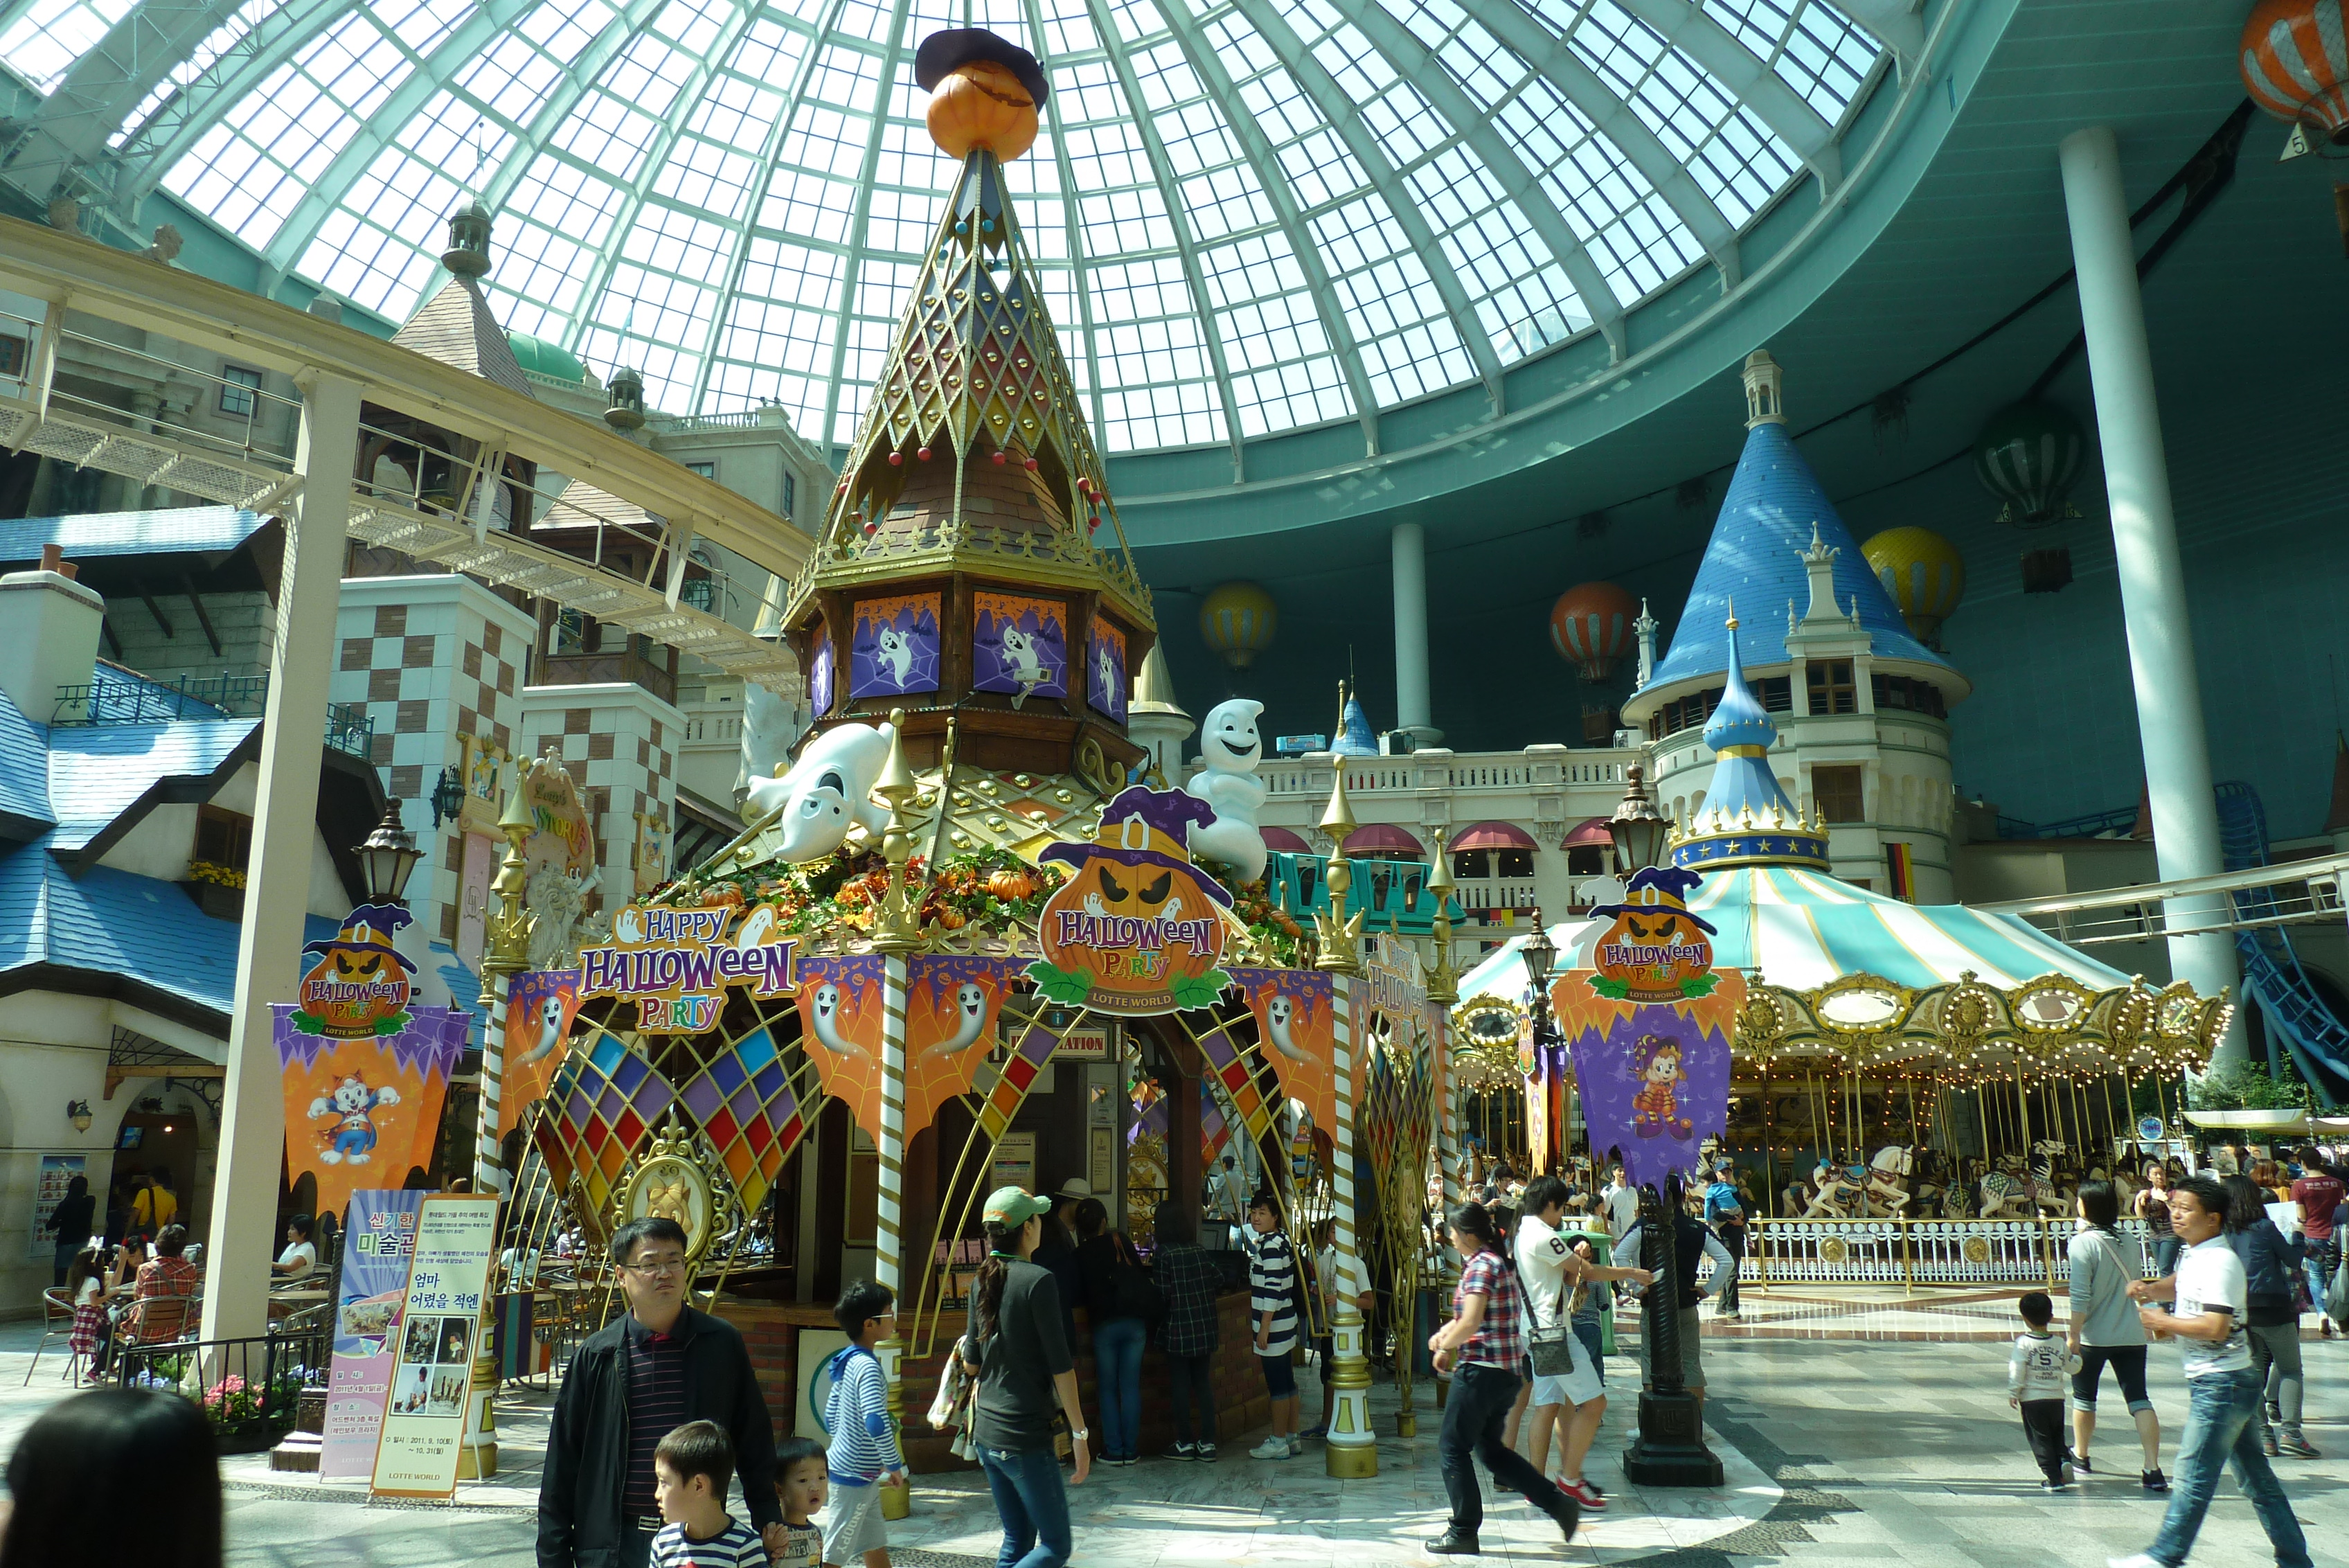
\includegraphics[width=0.40\textwidth]{photos/09/29/P1000380.jpg}}
\vspace{-24pt}
\end{wrapfigure}Lotte World is a theme park. According to Koreans, it is the biggest indoor theme park in Asia, which does not surprise me, because they are simply obsessed with superiority. As one presenter told us today during the Korean Business and Culture lecture, Koreans do not have fast food, they have \textit{aster} food. The park is located in Gangnam-gu ({\H 강남구}), close the the Olympic Park. It has two parts --- one big hall and the Magic Island, that is literally an island with a castle. Since this castle also dominates the Lotte World logo, when you see it, you can't stop wondering ``Hmm, this seems familiar!''. A little hint --- Disney.

I won't spend time describing the park, since it is a typical theme park with roller coasters, merry-go-rounds, thrill rides, water rides, big looping thingie, free fall tower, lots of junk food and little screaming kids. The hall with a indoor roller coaster is cool, especially because they managed to squeeze a lopping inside it. The sightseeing balloon ride around the hall was also fun --- a nice way to calm down after the endorphin and adrenaline shots on the roller coaster. The best attractions were on the Magic Island, though --- Gyro Swing and Atlantic Adventure really made my day. The first one is a giant pendulum with a rotating platform at the end, while the latter is a roller coaster with a launch start and few steep drops.

It was a nice day, I have to admit. Theme park is exactly the kind of activity that allows you to shut down your brain and just enjoy the thrill. You are screaming like a little kid, eating hamburgers for both breakfast and lunch and just having a good time. It is even better when you do it with a group of friends, because a shared experience is always better:)

Btw. there was one thing that really surprised me. LW was full of couples. That's not that surprising, right, but these couples were in many cases wearing the same clothes, or at least t-shirts/sweatshirts. I can't imagine that a European guy would do something like that. Not talking about the headbands with ears that both girls and guys were wearing. I guess that's simply Korea.

\begin{wrapfigure}{r}{0.51\textwidth}
\vspace{-12pt}\centering\fbox{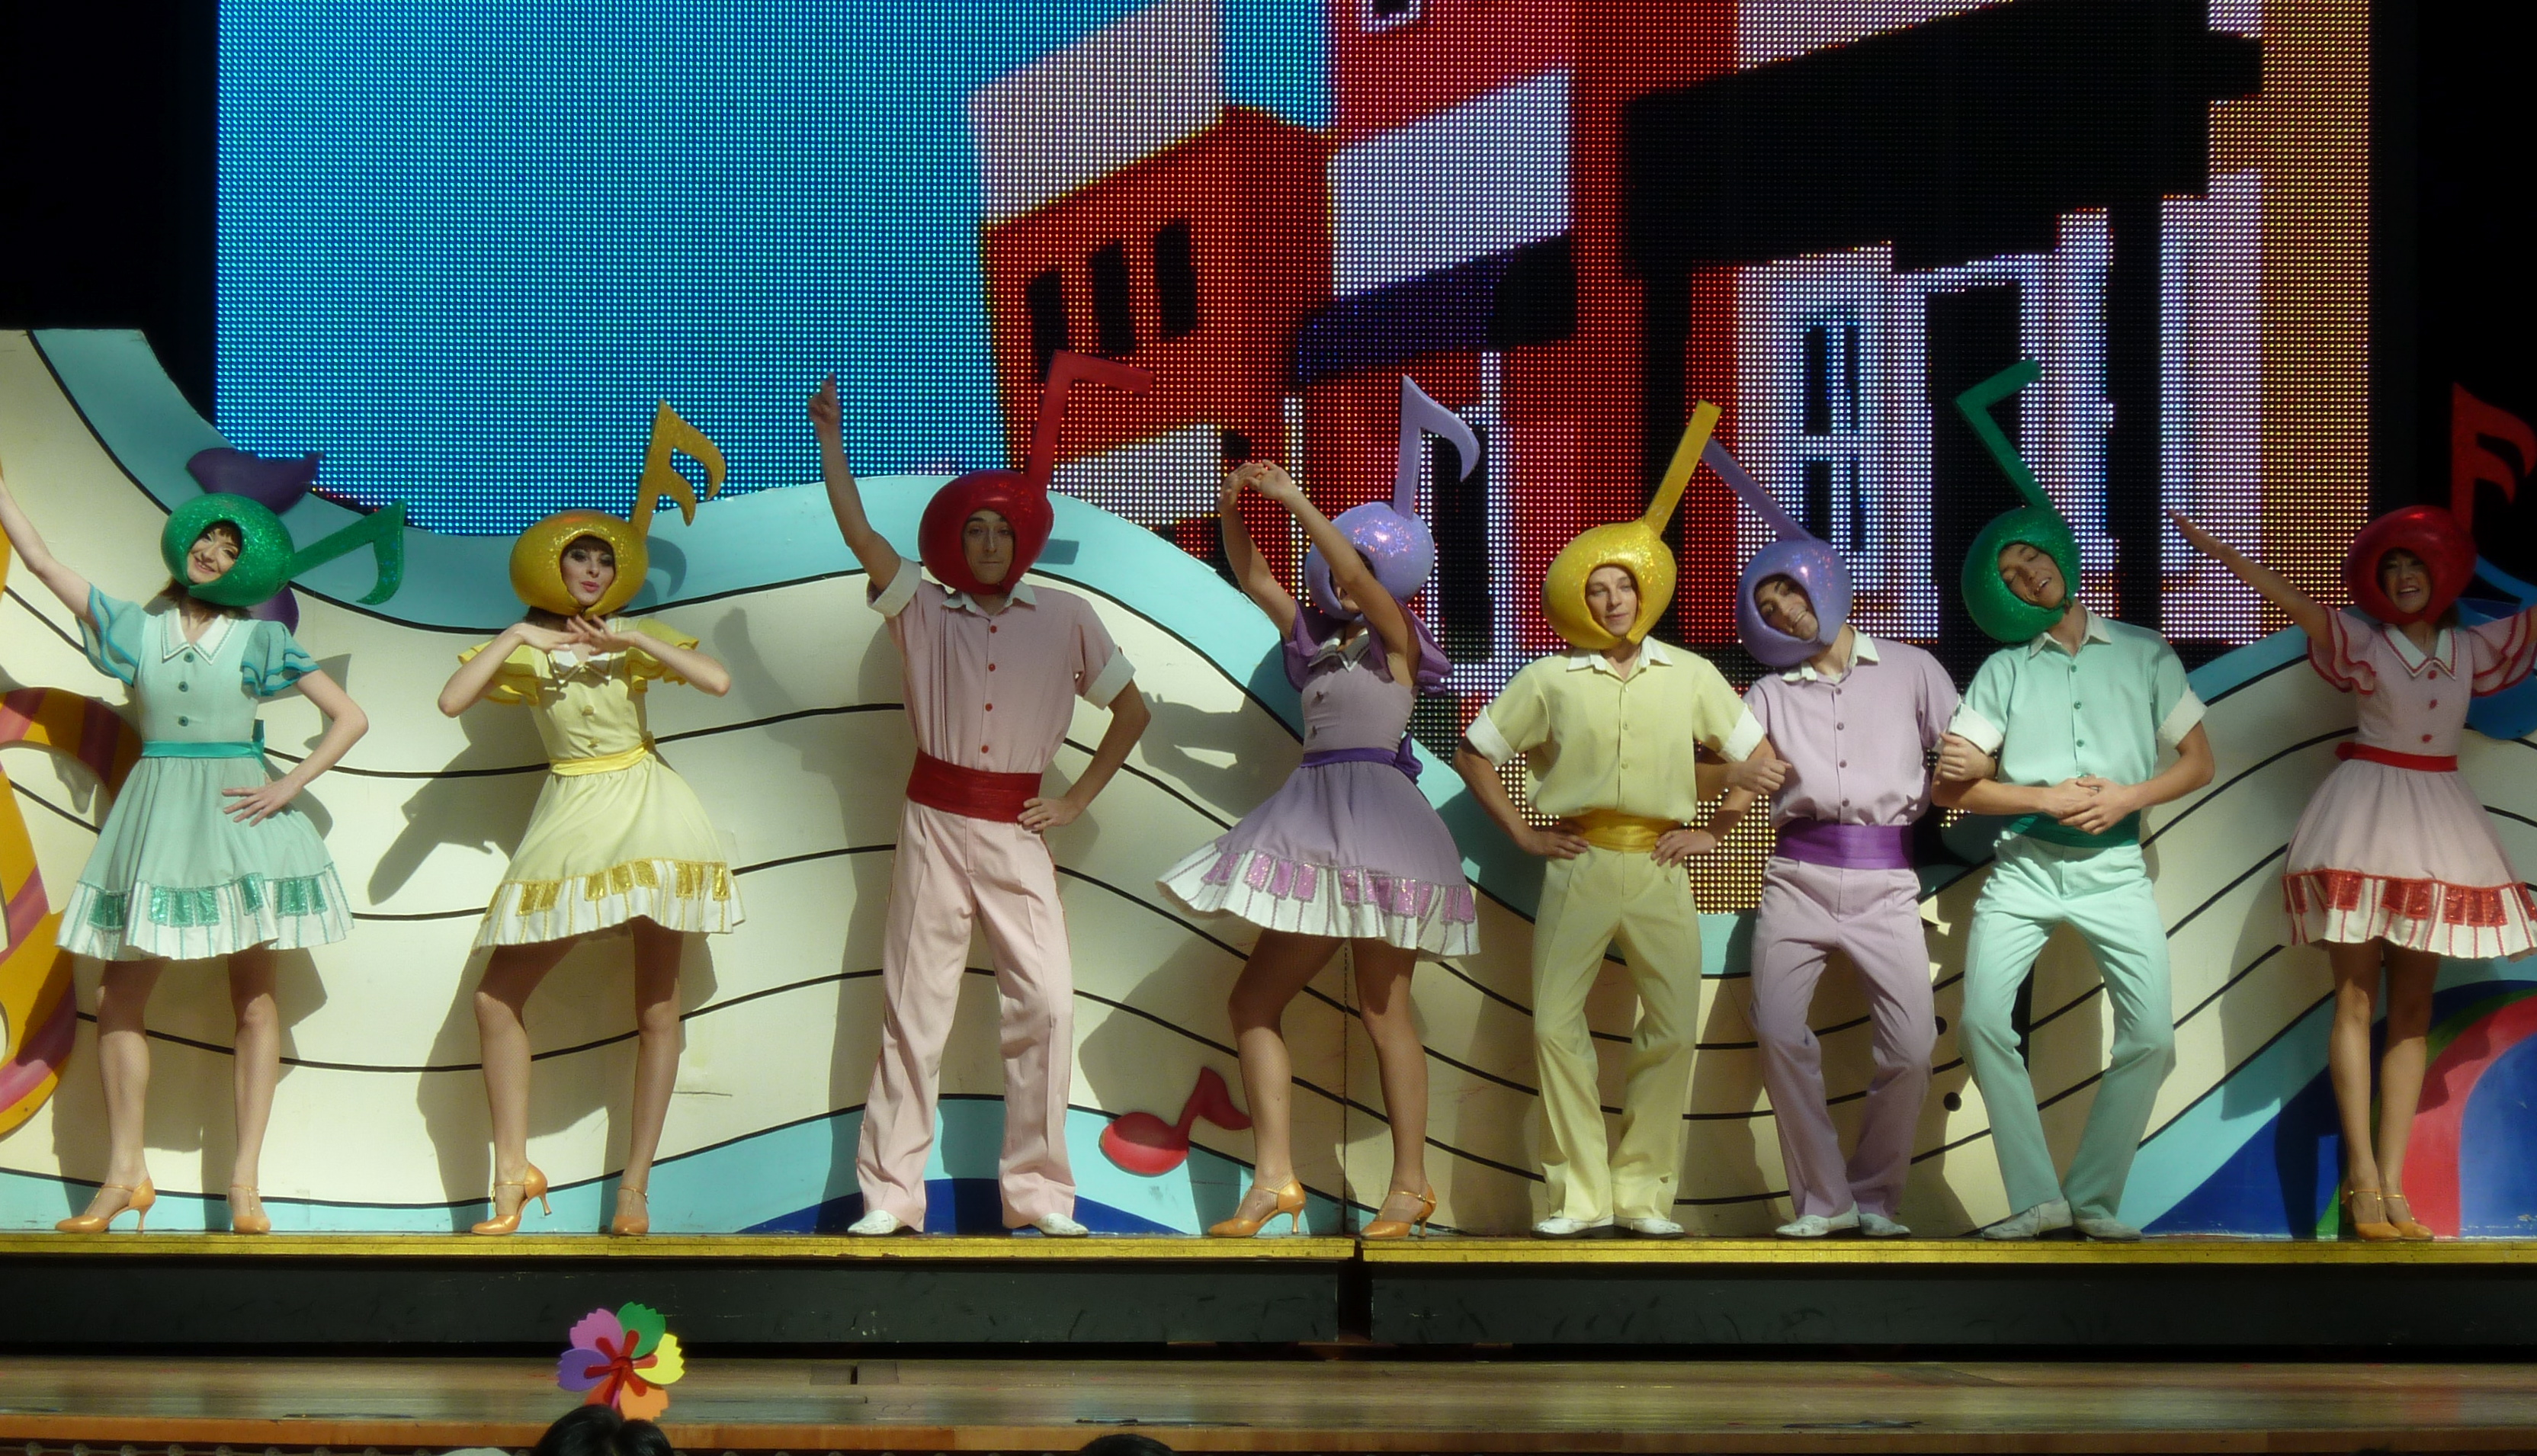
\includegraphics[width=0.5\textwidth]{photos/09/29/P1000432.jpg}}
\vspace{-24pt}
\end{wrapfigure}Oh yeah, I nearly forgot the Russian thing. Apparently, some Russian/Ukrainian dancers are working in LW as, well, dancers and performers. It was quite surprising to see white people performing in a Korean theme park, but I guess there is simply a limited market for ballet dancers in Europe:)

	\end{content}
\end{post}
